\subsection{Experiment Configuration}
\label{subsec:exp2-setup}

In each simulation run, one gNB and 20 UEs are used.
The UE count is fixed to 20 to keep per-step GPU memory and simulation wall-clock time within practical bounds on the evaluation hardware; scaling to denser deployments is outside the scope of this work.
The gNB antenna array is varied over $2\times2$, $4\times4$, and $8\times8$; each UE uses a fixed $2\times2$ array.
The simulations are tested in three different radio environments:
\begin{itemize}
    \item \textbf{free space}: $2$ GHz carrier, $35$ m gNB height, and UE
          distances from $50$ m to $1000$ m;
    \item \textbf{urban macro}: $3.5$ GHz carrier, $25$ m gNB height, and UE
          distances from $35$ m to $500$ m;
    \item \textbf{urban micro}: $28$ GHz carrier, $10$ m gNB height, and UE
          distances from $10$ m to $200$ m.
\end{itemize}
The carrier frequencies, antenna heights, and UE distance ranges are aligned with the 3GPP TR 38.901 reference deployment configurations \cite{tr38901}.
The 2~GHz carrier for the free-space baseline corresponds to the FR1 sub-3~GHz band; the 3.5~GHz urban macro carrier matches the primary 5G~NR band (n78, FR1); and the 28~GHz urban micro carrier represents the FR2 mmWave band (n257/n261).
The gNB heights of 25~m (urban macro) and 10~m (urban micro) follow the TR~38.901 UMa and UMi reference values respectively, while the 35~m free-space height is consistent with rural macro conventions.
The UE distance ranges are chosen to cover the minimum coupling distance and approximate cell radius defined for each scenario in TR~38.901 Table~7.2-1.
The single-cell, 20-UE configuration is consistent with the single-sector system-level evaluation methodology of TR~38.901 Table~A.1.
The free-space scenario is the baseline, the urban macro scenario represents a sub-6~GHz deployment, and the urban micro scenario represents the most demanding physical setting as it combines a mmWave carrier with geometry-sensitive, short-range links.
The 3D visualizations of these three environments are shown in Figure~\ref{fig:scenarios}.

\begin{figure}[t]
    \centering
    \subfloat[Free space.]{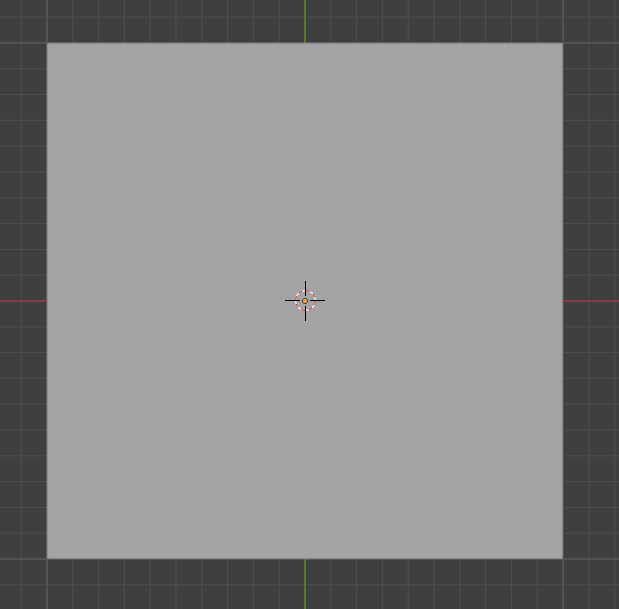
\includegraphics[width=0.32\linewidth]{images/free_space.png}\label{fig:scenario_free_space}}
    \hfill
    \subfloat[Urban macro.]{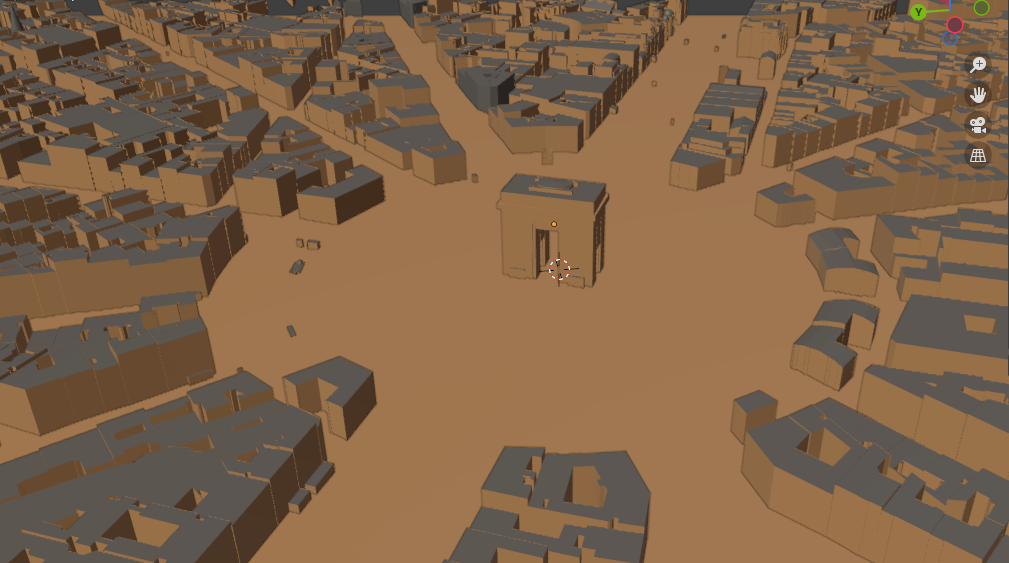
\includegraphics[width=0.32\linewidth]{images/urban_macro.png}\label{fig:scenario_urban_macro}}
    \hfill
    \subfloat[Urban micro.]{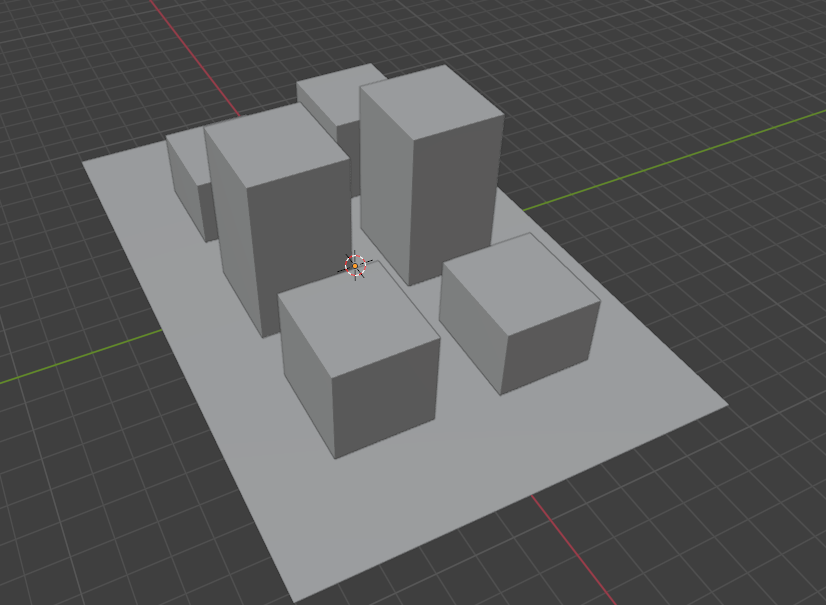
\includegraphics[width=0.32\linewidth]{images/urban_micro.png}\label{fig:scenario_urban_micro}}
    \caption{The three simulated radio environments.}
    \label{fig:scenarios}
\end{figure}

For scheduling UEs, a TDMA proportional fair scheduler, and full-buffer TDD slots are used.
On top of the realistic wireless channel model, different applications with different traffic loads are tested.
The traffic profile includes video, voice over IP (VoIP), social media, gaming, and FTP.
The per-application UE distribution — 12 (60\%), 2 (10\%), 2 (10\%), 1 (5\%), and 3 (15\%) for video, VoIP, social media, gaming, and FTP respectively — follows the traffic mix proportions reported in \cite{ericsson_mobility}, and is applied identically for both DL and UL.
The data rate for each application according to load levels are summarized in Table \ref{tab:exp2-offered-load}.

\begin{table*}[t]
    \centering
    \caption{Application data rate by application and load.}
    \label{tab:exp2-offered-load}
    \begin{tabular}{lrrrrrrr}
        \hline
        Application                & Flows                    & \multicolumn{2}{c}{Low} &
        \multicolumn{2}{c}{Medium} & \multicolumn{2}{c}{High}                                                                                       \\
        \cline{3-8}
                                   &                          & DL (Mbps)               & UL (Mbps) & DL (Mbps) & UL (Mbps) & DL (Mbps) & UL (Mbps) \\
        \hline
        Video                      & 12 DL / 12 UL            & 24.000                  & 0.300     & 96.000    & 1.200     & 300.000   & 3.750     \\
        VoIP                       & 2 DL / 2 UL              & 0.128                   & 0.032     & 0.256     & 0.064     & 2.000     & 0.500     \\
        Social                     & 2 DL / 2 UL              & 1.000                   & 0.050     & 10.000    & 0.500     & 40.000    & 2.000     \\
        Gaming                     & 1 DL / 1 UL              & 0.100                   & 0.025     & 1.000     & 0.250     & 10.000    & 2.500     \\
        FTP                        & 3 DL / 3 UL              & 3.000                   & 0.150     & 30.000    & 1.500     & 150.000   & 7.500     \\
        \hline
        Total                      & 20 DL / 20 UL            & 28.228                  & 0.557     & 137.256   & 3.514     & 502.000   & 16.250    \\
        \hline
    \end{tabular}
\end{table*}
